\documentclass[11pt,a4paper]{article}
\usepackage[english]{babel}
\usepackage[T1]{fontenc}

\usepackage{amsmath}
\usepackage{amsfonts}
\usepackage{amssymb}
\usepackage{fancyhdr}
\usepackage{a4wide} % Smaller margins = more text per page.
\usepackage[hidelinks]{hyperref}
\usepackage{graphicx}
\usepackage{epstopdf}
\usepackage{pdflscape}
\usepackage{multirow}
\usepackage{subcaption}
\usepackage{bbm}
\usepackage{color}
\DeclareMathOperator*{\argmax}{arg\,max}
\newcommand{\ml}[1]{\textcolor{red}{ML : #1}}
\pagestyle{fancy}
\begin{document}
\author{F\'elix Gontier $^1$, Catherine Lavandier $^2$, Pierre Aumond $^{2, 3}$\\Mathieu Lagrange $^1$, Jean-Francois Petiot $^1$}
\date{
$^1$\\
$^2$\\
$^3$
}
\title{Estimation of the perceived time of presence of sources in urban acoustic environment using deep learning techniques}
\maketitle


\begin{abstract}

\end{abstract}

\section{Introduction}
\label{sec:intro}
%- Du bruit au soundscape
%- La pleasantness premier axe sur les affects liés au soundscape
%- On a des modèles de pleasantness perceptifs qui font intervenir des temps de présence des sources
%- Peut-on à partir de la mesure physique faire des modèles de pleasantness sur la base d'indicateurs physiques?
%- Idée: si l'on fait de la reconnaissance de sources, on peut faire un meilleur modèle physique que les précédents
%- Première étape: On vérifie que le corpus créé est proche d'un corpus réel
%- Sur le corpus on fait de l'apprentissage profond
%- On compare le nouveau modèle physique deep en comparaison aux modèles physiques old school Cartazur (dimension purement niveau sonore) et Grafic (niveau sonore + Fréquence/sources)


\section{Methods}
\label{sec:methods}


\subsection{Perceptual validation}
\label{sec:pval}


\subsubsection{Sound scenes corpus}
\label{sec:pval_corp}

A first corpus is created to validate the use of simulated sound scenes in the development of pleasantness prediction models. It is based on recordings from one of the four soundwalks performed in~\cite{aumond2017}, including 19 locations in the 13th district of Paris. A classification of these scenes is proposed in~\cite{gloaguen2017} in terms of ambiance: \textit{park}, \textit{quiet street}, \textit{noisy street} and \textit{very noisy street}. For each of the 19 recordings 45 seconds of audio in a single channel are extracted that represent well the properties of their respective ambiances, and without single events overwhelming their overall perception. The resulting 45~s extracts are replicated to study perceptual differences between recorded and simulated scenes. The recordings are first annotated in terms of the following properties:

\begin{itemize}
\item Background sources that are present throughout the whole scene, and are associated with a sound level.
\item Sound events characterized for each occurrence by their source type, onset-offset and event-to-background ratio (EBR) in dB.
\end{itemize}

Sound scenes are then simulated using simScene~\cite{rossignol2015} with a database of extracts from recordings of isolated sound sources. This database is constructed from part of the LibriSpeech~\cite{panayotov2015} corpus for voices and Freesound\footnote{\url{https://freesound.org}} contributions for all other sources. The original recordings from 6 locations (P1, P3, P4, P8, P15 and P18) are chosen for perceptual comparison, as they explore diverse real-life situations with respect to environment categorization. All 6 recorded and 19 replicated scenes are normalized so that their playback sound level is the same as measured during recording, with a range from 63.9~dB to 79.4~dB.\\


\begin{figure}[h]
    \centering
     \begin{subfigure}[t]{0.33\textwidth}
        \centering
        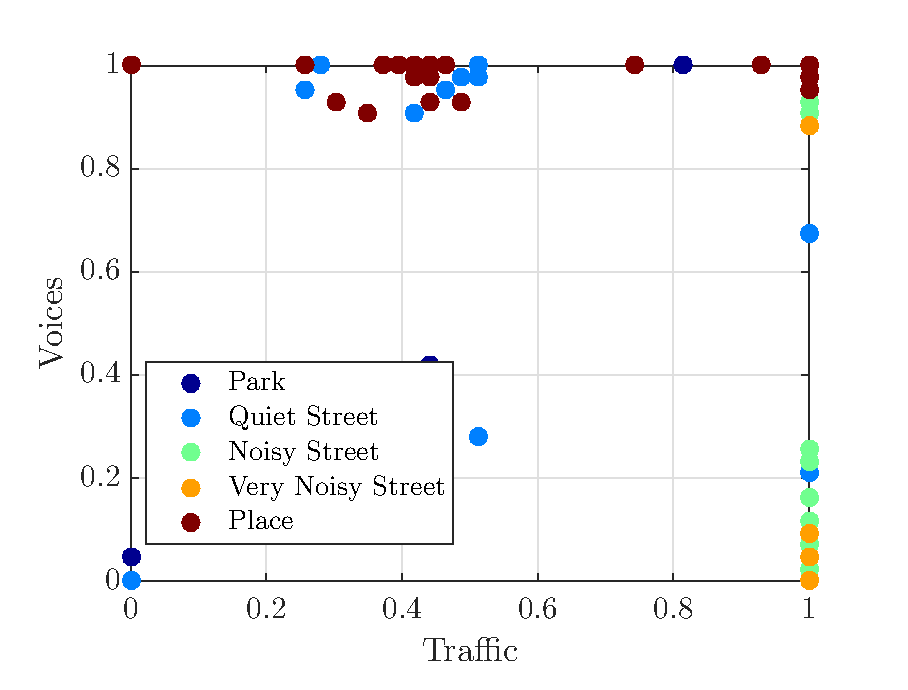
\includegraphics[width=\textwidth]{figures/tv_pres.eps}
    \end{subfigure}%
    \begin{subfigure}[t]{0.33\textwidth}
        \centering
        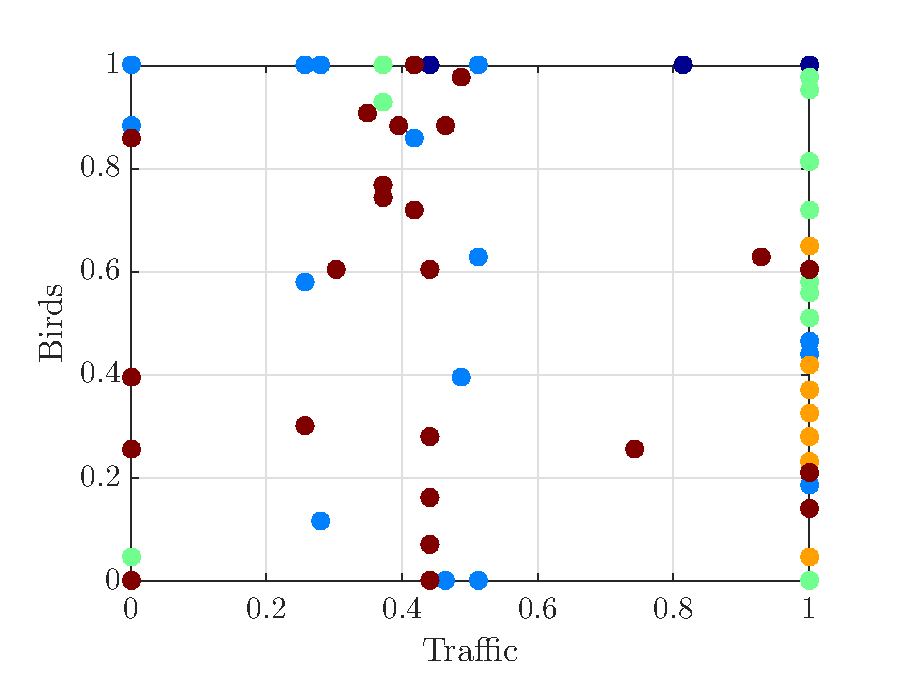
\includegraphics[width=\textwidth]{figures/tb_pres.eps}
    \end{subfigure}
    \begin{subfigure}[t]{0.33\textwidth}
        \centering
        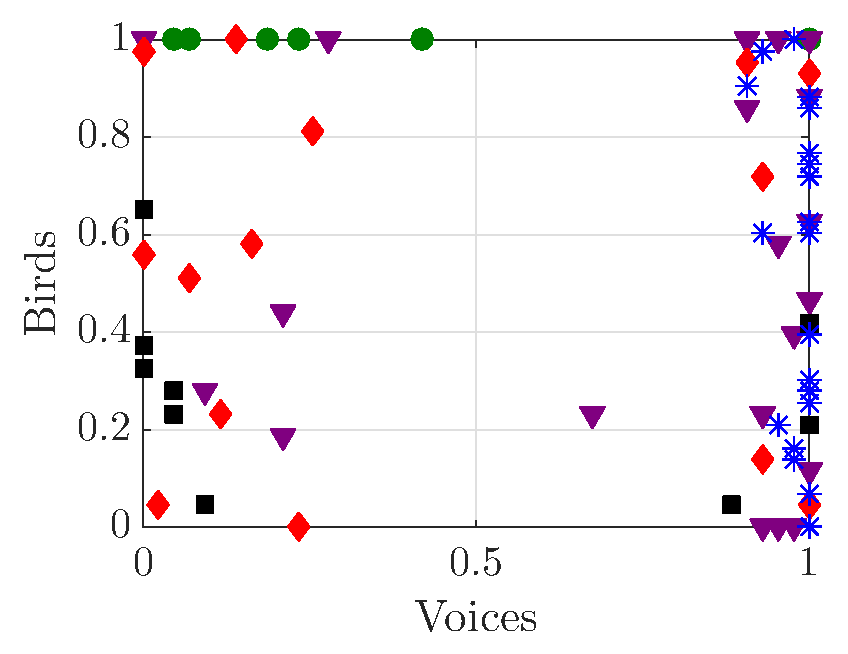
\includegraphics[width=\textwidth]{figures/vb_pres.eps}
    \end{subfigure}
    \caption{Estimated time of presence of traffic, voices and birds sources for the corpus of simulated scenes with automatically generated scenarios.}\label{fig:tvb_pres}
\end{figure}

To further study the perceptual properties of simulated scenes, the corpus is extended with 75 simulated scenes corresponding to new scenarios. Because of the lack of large isolated sources datasets, we choose to restrict the scene composition to 3 sources: \textit{traffic}, \textit{human voices} and \textit{birds}. Considering the aim of the study, newly generated scenarios should cover most real-life situations while remaining perceptually plausible. Thus, statistics on background and event properties are extracted for each of the three sources from annotations presented in~\cite{gloaguen2017}. These statistics include, conditionally to the ambiance:

\begin{itemize}
\item The probability of appearance of a given source in the scene, for which events and backgrounds are considered separately,
\item Event-to-background ratios in dB for all events and backgrounds besides the first, in the form of normal distributions,
\item The inter-onset of event occurrences in seconds, also in the form of normal distributions.
\end{itemize}

Adjustments are made on the variance of the considered properties to better cover possible scenarios, and the EBR of voice events, mostly read English recordings, are reduced to improve realism. An additional \textit{place} ambiance is added with properties derived empirically from available data. Diverse new scenarios are then generated by sampling the background and event properties distributions. For each scene the time of presence for the traffic, voice and bird sources is estimated using indicators proposed in~\cite{gontier2018}, and 75 scenes are chosen to maximize pairwise distance in the resulting 3-dimensional space. This is shown in Figure~\ref{fig:tvb_pres}. The playback sound level is also conditioned on the ambiance according to typical sound levels in urban context shown in Figure~\ref{fig:amb_levels}, and ranges from 46.6~dB to 77.1~dB.\\

The experiment corpus thus totals 100 scenes: 6 recorded and 19 replicated scenes from the Grafic project, and 75 simulated scenes.

\begin{figure}[!h]
    \centering
    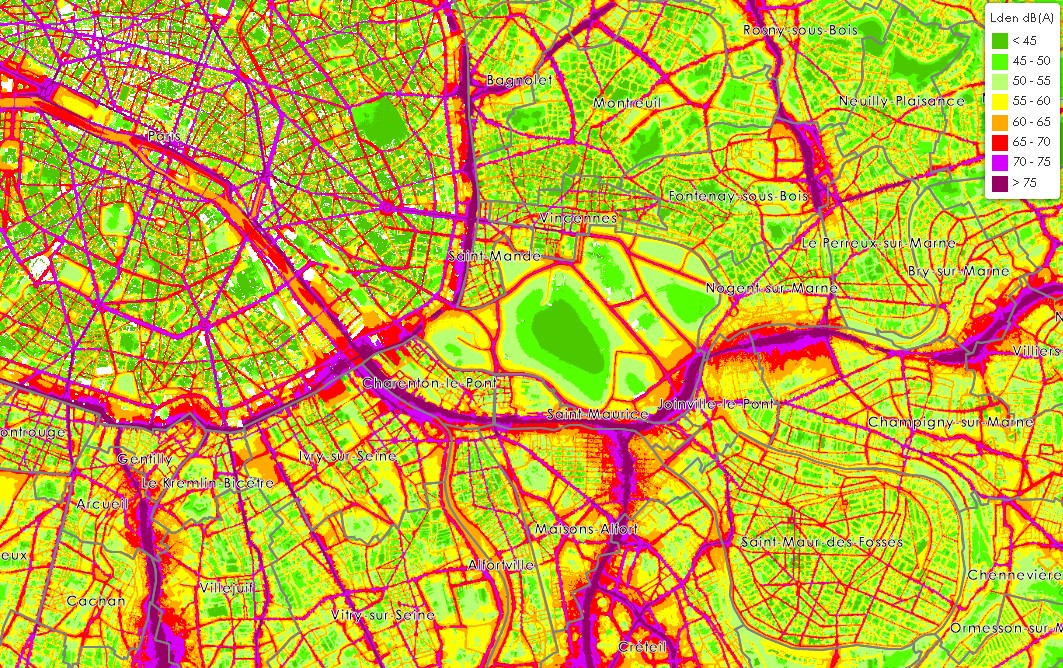
\includegraphics[width=0.8\textwidth]{figures/lvls.jpg}
    \caption{Example of sound level scale a function of the environment for new simulated scenes. TODO CITE}\label{fig:amb_levels}
\end{figure}


\subsubsection{Experiment}
\label{sec:pval_exp}

A perceptual experiment is conducted where participants are asked to evaluate sound scenes in terms of 9 criteria represented by 11 point (0-10) scales. These scales are presented in french and translated in this report using standard terminology. The first 5 scales relate to general properties of the scene:
\begin{itemize}
\item Pleasantness: \textit{Unpleasant - Pleasant} (\textit{D\'esagr\'eable - Agr\'eable}) - P
\item Liveliness: \textit{Inert, amorphous - Lively, eventful} (\textit{Inerte, amorphe - Anim\'e, mouvement\'e}) - L
\item Overall loudness: \textit{Quiet - Noisy} (\textit{Silencieux - Bruyant}) - OL
\item Interest: \textit{Boring, uninteresting - Stimulating, interesting} (\textit{Ennuyeux, inint\'eressant - Stimulant, int\'eressant}) - I
\item Calmness: \textit{Agitated, chaotic - Calm, peaceful} (\textit{Agit\'e, chaotique - Calme, tranquille}) - C
\end{itemize}


These quantities are typically studied in the perceptual characterization of sound scenes~\cite{axelsson2010, aumond2017, nilsson2007}. While this work focuses on pleasantness, including other dimensions can be useful to verify the relevance of the data in relation to previous work.\\

Previous studies show that pleasantness is mainly influenced by the activity of three sources: traffic, human voices and birds. The perception of source activity can be linked to notions of dominance, time of presence, or emergence. We choose the perceptual time of presence, that is the percentage of time for which the corresponding source is heard, as the activity descriptor for this study. The influence of traffic on pleasantness is further separated into that of background and emergent events. Thus, 4 additional questions are presented:
\begin{itemize}
\item Sound level of passing vehicles: \textit{Very low - Very high} (\textit{Tr\`es faible - Tr\`es fort}) - $L_{T, p}$,
\item Time of presence of Traffic, Voices, Birds: \textit{Never - Continuously} (\textit{Jamais - Continuellement}), resp. $T_{T, p}$, $T_{V, p}$ and $T_{B, p}$
\end{itemize}

Prior to the test, participants are given a short verbal introduction and the interface is introduced before the test to ensure that the quantities are well understood. Although the corpus is comprised of 100 sound scenes, participants only evaluate 50 scenes: all listen to the 6 recorded and 19 replicated sound scenes, then to 25 of the 75 simulated with new scenarios. The selection of simulated scenes is done so that all scenes in the sub-corpus are evaluated by the same number of participants. A random pre-generated listening order is used to attenuate ordering effects, although all participants are first presented with the most quiet then most noisy of the recorded scenes (resp. P3 and P15) to calibrate their answers. For the remainder of the corpus all participants experience different scene ordering. Participants can only listen to each scene once, and have to answer all questions and listen to the full extract before proceeding to the next.\\

The scenes are played at a given sound level as discussed in Section~\ref{sec:pval_corp}, through the same computer and sound card configurations. Beyerdynamics DT-990 Pro headphones are used for all participants. These headphones are calibrated in a semi-anechoic chamber, resulting in a relation between playback Leq and LAeq and sound card output voltage for pink noise. This ensures that correctly scaled scenes will be heard at the desired sound level by listeners.\\

A total of 23 students aged 22 to 23 including 16 males and 7 females at Ecole Centrale de Nantes completed the test. All gave consent prior to the experiment.

\subsection{Indicators for pleasantness prediction}
\label{sec:inds}

Several indicators are computed from the audio signals that are found in previous studies~\cite{aumond2017, gontier2018, ricciardi2014} to correlate well with perceptual parameters.\\

First, indicators can be computed directly from the mixed audio, without the need for information about the composition of the scene, \textit{i.e.} source activity and level. Typically this includes indicators derived from sound level measurements. For this study the following are computed with 1~s (slow) measurements using the Matlab ITA-toolbox~\cite{itatoolbox2017}:

\begin{itemize}
\item Z-weighted $L_{eq}$ and A-weighted $LA_{eq}$ equivalent sound levels in dB and dBA respectively.
\item $L_{10}$, $L_{50}$ and $L_{90}$: 10th, 50th and 90th percentiles of the Z-weighted sound level. The $L_{10}$ is associated to events and the $L_{90}$ to background activity, while the $L_{50}$ is a measurement of the overall sound level.
\item $LA_{50}$: 50th percentile of the A-weighted sound level, with similar properties as the $L_{50}$.
\item $L_{50, 1kHz}$: 50th percentile of the Z-weighted sound level for the 1kHz frequency band, also a good descriptor of the overall sound level of the scene.
\item $LA_{10}-LA_{90}$: Emergence indicator included in the pleasantness model in~\cite{ricciardi2014}.
\end{itemize}

The time and frequency second derivative ($TFSD$) is introduced in~\cite{aumond2017} as a descriptor of source activity. To provide a baseline for pleasantness prediction the $TFSD$ is computed for the 4kHz band and 125~ms measurements ($TFSD_{4kHz(1/8s)}$) to represent birds, and for the 500Hz band with 1~s measurements ($TFSD_{500Hz(1s)}$) to represent voices.\\

The simulation process outputs ground truth source contributions in the form of separate channels. Additional indicators are computed on the separated audio signals for the traffic, voices and birds sources:

\begin{itemize}
\item $L_{eq, s}$: Equivalent sound level for source $s$
\item $\Delta L_{s}$: Source emergence, taken as the difference between the equivalent sound level of source $s$ and that of all other sources combined
\end{itemize}

Next, the $\hat T_s(\alpha, \beta)$ time of presence approximation proposed in~\cite{gontier2018} is computed. $\hat T_s(\alpha, \beta)$ is based on a binary source emergence model computed on the third-octave band emergence $\Delta_s(t, f) = L_s(t, f) - L_{\bar{s}}(t, f)$. It is parametrized by $\alpha$ and $\beta$ thresholds:

\begin{align}
\hat T_s(\alpha, \beta) &= \frac{1}{N_t}\sum_{t = 1}^{N_t}\mathbbm{1}\left[ \frac{\sum_{f = 1}^{N_f}\Delta_s(t, f)\mathbbm{1}_{\Delta_s(t, f)>\alpha}}{\sum_{f = 1}^{N_f}\mathbbm{1}_{\Delta_s(t, f)>\alpha}}>\beta \right]\\
\alpha_{opt},\beta_{opt} &= \argmax_{\alpha, \beta}\frac{1}{N_s}\sum_{s = 1}^{N_s}r\left(T_{s, p}, T_s(\alpha, \beta)\right)
\end{align}

where $r$ is the Pearson's correlation coefficient, $s$ denotes the sound source, $t$ is the time frame and $T_{s, p}$ correspond to the perceptual time of presence assessments. The optimal threshold values are found as $\alpha_{opt} = -14dB$ and $\beta_{opt} = -7dB$. This means that to be considered heard in a given time frame, the source has to be emergent by more than $-7dB$ on average on bands where its level is at least $14dB$ below other sources.\\

In the remainder of this paper, the subscript $s$ is replaced with the corresponding source initial: $T$ for traffic, $V$ for voices and $B$ for birds.




\subsection{Indicator prediction through deep learning}
\label{sec:deep}

\subsubsection{Learning corpus}
\label{sec:deep_corp}

To train deep learning architectures for source recognition, a larger corpus is constructed. It is composed of two datasets of simulated scenes:
\begin{itemize}
\item The development set containing 400 45~s scenes (total 5 hours) which is used during the training process,
\item The evaluation set containing 200 45~s scenes (total 2.5 hours) which is used to compute the performance of the trained model and its generalization capabilities.
\end{itemize}

The generation procedure is the same for both datasets, and is equivalent to that of the simulated sub-corpus considered for the perceptual test in Section~\ref{sec:pval_corp}. Only traffic, human voices and birds sources compose the sound scenes due to the low number of available samples and recording annotations for other sources. The isolated samples database is split in the same proportions as the two datasets: two-thirds for the development set and the remaining one-third for the evaluation set. As a result, while the generation process is the same for both corpora both the scenarios and samples are different.\\

The sensors implemented as part of the Cense project provide fast measurements of sound levels for each third-octave band in the $20~Hz - 12.5~kHz$ range in their normal operation~\cite{ardouin2018, gontier2017}. Thus, a prediction model should take as input the same representation. Third-octave spectra are computed for 125~ms frames and 29 frequency bands of the mixed sound scenes. Inputs are then obtained by splitting the resulting spectrograms into frames with a 1~s duration, which is considered a relevant scale for perception. The input frames of dimension 29x8 are then processed independently in this study.\\

Target outputs are associated to each input frame to train the model. Based on previous work the time of presence of traffic, voices and birds can be approximated by the $\hat T_s(\alpha, \beta)$ indicator. Thus, the source presence values before averaging along time can be used as weak labels. Alternatively, it is possible to perform sound level estimation using ground truth labels. Though, this regression task is difficult to learn compared to source detection, and did not result in better time of presence estimations in our experiments.

\subsubsection{Model architecture}
\label{sec:deep_mdl}

A deep learning model is implemented and trained for the source presence prediction task, with the architecture shown in Figure~\ref{fig:deep_arch}. The model includes 4 blocks of convolutional layers followed by LeakyReLU activations. The convolutional layers have respectively 128, 64, 32 and 32 output maps, \textit{i.e.} channels, and a common kernel size of 5x5. The output of the last block is flattened then goes through a fully connected layer with output size 3. A final sigmoid activation is used to obtain outputs in the 0-1 range. The resulting 3 values correspond to the presence of traffic, voices and birds respectively, and are compared during training to presence labels given by $\hat T_s(\alpha, \beta)$ using a binary cross-entropy cost function:
\begin{equation}
L(y, \hat y) = -\sum_s y_s log\left(\hat y_s\right) + (1-y_s) log\left(1-\hat y_s\right)
\end{equation}
where $s$ is the source, $y_s$ and $\hat y_s$ are the target and predicted presence for source $s$ in the 0-1 range. This loss function is minimized using the Adam algorithm~\cite{kingma2015} on batches of 1~s examples.\\

\begin{figure}[!h]
    \centering
    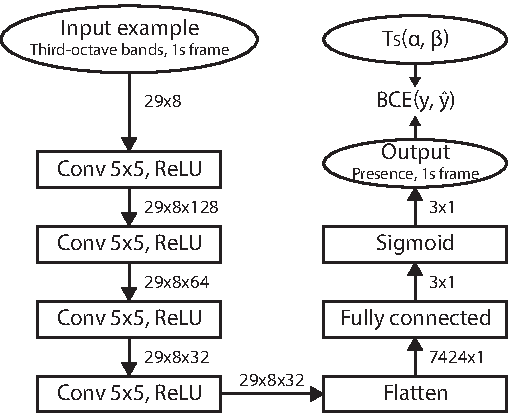
\includegraphics[width=0.8\textwidth]{figures/deep_arch.pdf}
    \caption{Architecture of the deep learning model used for source presence prediction.}\label{fig:deep_arch}
\end{figure}

When using the model's outputs to estimate the time of presence of sources, a threshold of 0.5 is used to obtain binary presence values.



\section{Results}
\label{sec:results}


\subsection{Perceptual validation}
\label{sec:perc}
%=> 3.1, 3.2

Participants evaluate each scene on criteria coded on 11-point discrete scales. Many statistical tools assume that the studied data follows continuous, single mode distributions. It is thus important to first verify that no distinct groups of participants can be obtained from perceptual assessments. A hierarchical clustering analysis of the participants is performed for the 25 scenes in the commonly evaluated sub-corpus, and shown in Figure~\ref{fig:hclusters}. No clear separation into groups is found, as a result the assessment distributions are assumed to be single-mode and their means can be used for further analysis.\\

\begin{figure}[!h]
    \centering
    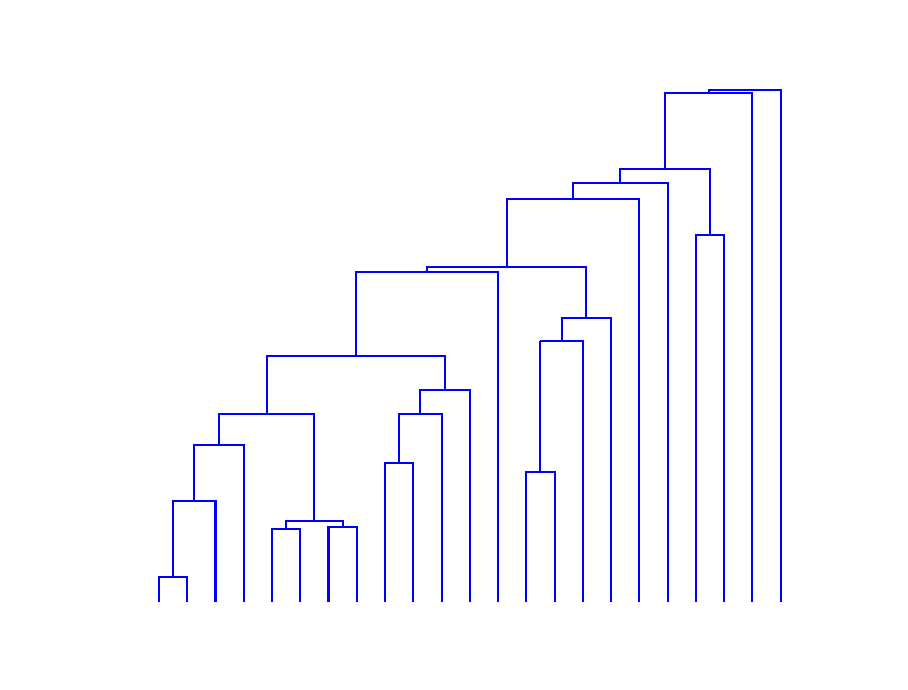
\includegraphics[width=\textwidth]{figures/subj_gr.eps}
    \caption{Dendrogram of the hierarchical clustering of participants on the first 25 scenes of the test. No distinct groups are visible.}\label{fig:hclusters}
\end{figure}



The perceptual responses of the 6 recorded and corresponding replicated scenes are then compared. Table~\ref{tab:ogrep} shows the mean differences between assessments for pairs of scenes with equivalent scenarios. Kolmogorov-Smirnov statistical tests are implemented for each scene and perceptual scale to outline significant differences between assessment distributions, which are shown in bold. Pleasantness is found to differ between the two groups only for one location, P4, which can be explained by high discrepancies in the perceptual time of presence of traffic and voices. For this location, the background traffic in the recorded scene varies along time, it is louder in the first half of the scene than in the second half. Replicating this scene using simScene imposes a constant sound level for background sources. Thus, the background traffic is louder in the replicated scene than it is in the recording for about half of its duration. To a lesser extent the same issue explains the large difference in assessed time of presence of voices in the location P3, but as voices have a less distinct influence on pleasantness this is not reflected directly. Discrepancies can also be interpreted by the choice of isolated samples, which is semi-random and based on a high-level source taxonomy. For example, no difference is made during annotation between child or adult speech, or depending on its expressiveness. Overall, no consistent difference between the perception of recorded and replicated scenes is found for the studied points. Thus, the proposed hypothesis that recorded and replicated scenes generate the same perceptual responses cannot be rejected.\\

\begin{table}[h]
\centering
\caption{Mean differences of perceptual assessments between original and replicated sound scenes. Significantly different distributions as per a Kolmogorov-Smirnov test are in bold (n=23, p<0.05)}
\label{tab:ogrep}
%\resizebox{\columnwidth}{!}{
\begin{tabular}{ c | c c c c c c c c c }
\hline
	 & P & L & OL & I & C & $L_{T, p}$ & $T_{T, p}$ & $T_{V, p}$ & $T_{B, p}$ \\ \hline
	P1 & 0.43 & \textbf{-1.65} & -1.04 & 0.43 & 0.13 & -0.91 & 0.39 & -2.09 & 0.61 \\
	P3 & 0.26 & -0.43 & 0.30 & -1 & 0.30 & 0.35 & 1.04 & \textbf{-4} & 0.22 \\
	P4 & \textbf{0.91} & 0 & \textbf{-1.83} & 0.48 & 1.30 & -0.96 & \textbf{-5.22} & \textbf{1.43} & 0.04 \\
	P8 & 0.26 & \textbf{-1.65} & -0.87 & -0.96 & 0.65 & \textbf{-2.04} & -0.91 & 0.09 & \textbf{-1.43} \\
	P15 & -1.35 & 0.52 & 0.52 & -1.17 & 0.09 & 0.61 & 0.13 & \textbf{1.96} & \textbf{-2.74} \\
	P18 & 1.13 & -0.30 & -1.17 & -0.43 & 1.39 & -1.04 & -1.83 & 0.83 & \textbf{1.30} \\ \hline
\end{tabular}
%}
\end{table}

To validate the use of simulated sound scenes with new scenarios as well as reduced source complexity in the development of prediction models, the perceptual space generated by the experiment's five general scales is studied. It is obtained by performing a principal components analysis (PCA) on the corresponding perceptual responses at the scene level. Figure~\ref{fig:pspace} compares the results for scenes based on recordings (left, n=25) and new scenarios (right, n=75). The generated spaces are similar, with only overall loudness and pleasantness axes slightly rotated between the two corpora. For both sets the variance explained by the first two components is similar (resp. 79.4\% - 18.1\% and 79.6\% - 15.2\%). Furthermore, these representations are comparable to those found in previous work on perceptual dimensions~\cite{axelsson2010, cain2013}. Thus, the use of simulated scenes based on both real and new scenarios does not result in major differences in the relations between perceptual quantities. Additionally, assessments for each scene are projected onto the PCA space and represented in Figure~\ref{fig:pspace} as dots. The space covered by scenes based on new scenarios covers that of the studied real-life environments, further demonstrating the efficiency of the scene generation procedure in terms of diversity.\\

Discrepancies between projections of original and replicated scenes are highlighted in Figure~\ref{fig:pspace}a by arrows, and the standard deviation of assessments is represented by ellipses for one scene. The projections of assessment distributions consistently overlap for all pairs of recorded and replicated scenes, not shown here for clarity. This illustrates the results in Table~\ref{tab:ogrep} where perceptual assessments were not found to differ significantly overall.\\

% FIGURE
\begin{figure}[h]
    \centering
     \begin{subfigure}[t]{0.55\textwidth}
        \centering
        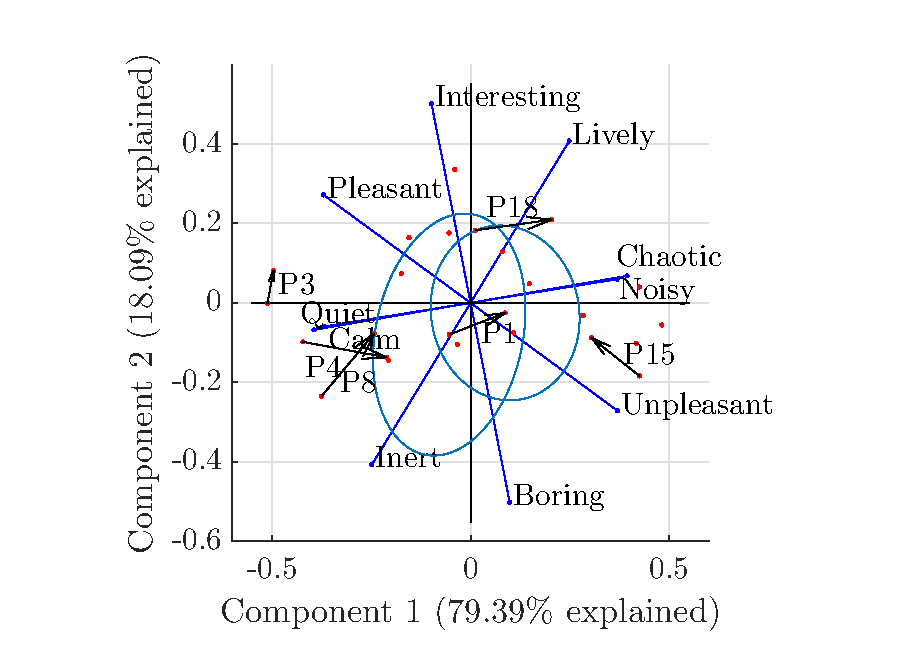
\includegraphics[width=\textwidth]{figures/pca_p1.eps}
    \end{subfigure}%
    \begin{subfigure}[t]{0.5\textwidth}
        \centering
        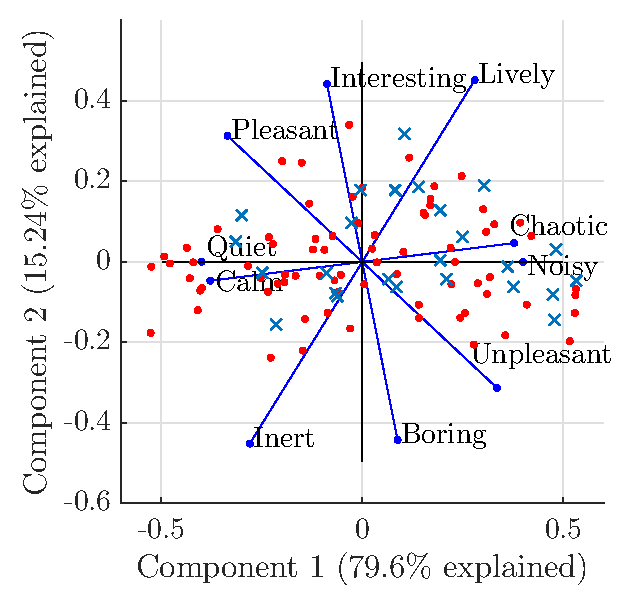
\includegraphics[width=\textwidth]{figures/pca_sim.eps}
    \end{subfigure}
    \caption{Principal components analysis (first two components) of the four general questions at the assessment level (n=252). Each dot represent the projection of one scene on the resulting space. The components space is distorted compared to the litterature.}\label{fig:pspace}
\end{figure}

\subsection{Baseline pleasantness models}
\label{sec:base}
%=> 3.3, 4.2


\subsubsection{Perceptual models}
\label{sec:base_perc}

\begin{table}[h]
\centering
\caption{Pearson's correlation coefficients between perceptual scales at the scene level (n=100, *: p<0.05, **: p<0.01)}
\label{tab:percc}
%\resizebox{\columnwidth}{!}{
\begin{tabular}{ c | c c c c c c c c c }
\hline
	 & P & L & OL & I & C & $L_{T, p}$ & $T_{T, p}$ & $T_{V, p}$ & $T_{B, p}$ \\ \hline
	P & 1 & -0.53** & -0.89** & 0.66** & 0.88** & -0.82** & -0.76** & 0.05 & 0.57** \\
	L &  & 1 & 0.76** & 0.06 & -0.78** & 0.39** & 0.17 & 0.60** & -0.36** \\
	OL &  &  & 1 & -0.39** & -0.96** & 0.71** & 0.59** & 0.17 & -0.45** \\
	I &  &  &  & 1 & 0.35** & -0.55** & -0.67** & 0.38** & 0.48** \\
	C &  &  &  &  & 1 & -0.67** & -0.55** & -0.24* & 0.48** \\
	$L_{T, p}$ &  &  &  &  &  & 1 & 0.79** & -0.15 & -0.41** \\
	$T_{T, p}$ &  &  &  &  &  &  & 1 & -0.35** & -0.42** \\
	$T_{V, p}$ &  &  &  &  &  &  &  & 1 & -0.21* \\
	$T_{B, p}$ &  &  &  &  &  &  &  &  & 1 \\ \hline
\end{tabular}
%}
\end{table}

We first study the relations between perceptual scales with respect to existing work. Table~\ref{tab:percc} shows the Pearson's correlation coefficients at the scene level, that is on the mean responses for each scene. The resulting values are consistent with the literature~\cite{aumond2017, gontier2018}, both between general scales as discussed in the previous section and for the relations to source contributions. Pleasantness (P) is mainly influenced negatively by overall loudness and traffic and positively by birds. In previous studies a small positive contribution of voices to pleasantness was found, while no direct relation is visible from the data gathered. This can be explained by the choice of speech samples used during generation, which consist of read audiobooks extracts and thus may sound unnatural in the considered urban environments. Liveliness (L) is here negatively though weakly (r<0.4) correlated with the presence of birds, while no significant relation was found in previous studies.\\

Relations between source-specific parameters are also weak with the exception of traffic being negatively correlated with birds. The perceived sound level of passing vehicles $L_{T, p}$ is a potential alternative to the time of presence of traffic $T_{T, p}$. Except for the interest (I) it displays higher correlations with general scales and lower correlations with other source-specific parameters.\\

As a baseline for pleasantness prediction, multilinear models are built as a function of both the overall loudness (OL) and source-specific parameters. To ensure that no multi-collinearity is present between predictors a variance inflation factor (VIF) test is performed prior to model regression. Only models for which all predictors verify $VIF<5$ are considered valid. The best resulting models with statistically significant estimates ($p<0.05$) for all predictors are:

\begin{align}
\hat P_{p1} &= 8.56 - 0.63~OL - 0.20~L_{T, p} + 0.11~T_{V, p} + 0.14~T_{B, p}\\
\hat P_{p2} &= 8.99 - 0.67~OL - 0.15~T_{T, p} + 0.08~T_{V, p} + 0.12~T_{B, p}
\end{align}

Both models have very similar formal expressions, with important negative contributions of the overall loudness and traffic activity. A small positive contribution of the time of presence of voices is also found despite no significant correlation.\\

Table~\ref{tab:percm} summarizes performance metrics computed for the two models. $\hat P_{p1}$ and $\hat P_{p2}$ display similar estimation errors as well as no significant difference in adjusted $R^2$ and correlation to assessed pleasantness. The mean standard deviation of pleasantness assessments for this experiment is about 1.77, thus perceptual models are considered accurate with about 0.6 RMSE on the 10-point scale.

\begin{table}[t]
\centering
\caption{Performance of perceptual models for pleasantness prediction (**: p<0.01).}
\label{tab:percm}
%\resizebox{\columnwidth}{!}{
\begin{tabular}{ c | c | c | c }
\hline
	 & $RMSE$ & $R^2_{adj}$ & $r$ \\ \hline
	$\hat P_{p1}$ & 0.59 & 0.91 & 0.95** \\
	$\hat P_{p2}$ & 0.61 & 0.90 & 0.95** \\ \hline
\end{tabular}
%}
\end{table}

\subsubsection{Physical models}
\label{sec:base_phys}

The analysis of physical indicators is done using the arithmetic mean of subjective assessments over all participants for replicated and simulated scenes. Two scenes containing only one source are excluded for implementation concerns, resulting in $n=92$ scenes.\\

Table~\ref{tab:physc} shows the Pearson's correlation coefficients between computed physical indicators and perceptual assessments. First, all measurements of global sound levels correlate well (r>0.9) with the perceived overall loudness. Regarding source-specific perceptual parameters, the $L_{eq, s}$ correlates consistently well with the $T_{s, p}$ of corresponding source. Conversely, the emergence $\Delta L_s$ fails to represent the perceived bird activity, and correlations are weaker for other sources. The proposed estimates of the time of presence $\hat T_s(\alpha, \beta)$ show strong correlations to their perceptual counterparts (r>0.8), along with good source discrimination properties. They are also better predictors than the $TFSD_{500Hz, 1s}$ and $TFSD_{4kHz, 1/8s}$ indicators for voice and bird activity. Interestingly, the perceived sound level of passing vehicles $L_{T, p}$ is best represented by the $L_{10}$. In perceptual models including the sound level of traffic events, the global $L_{10}$ may thus be a sufficient predictor without a source separation and level estimation algorithm.\\

\begin{table}
\centering
\caption{Pearson's correlation coefficients between physical and perceptual indicators (n = 92, *: p<0.05, **: p<0.01). Non significant correlations at the 5\% threshold are noted NS.}
\label{tab:physc}
\resizebox{\columnwidth}{!}{
\begin{tabular}{ c | c c c c c | c c c c }
\hline
	 & P & L & OL & I & C & $L_{T, p}$ & $T_{T, p}$ & $T_{V, p}$ & $T_{B, p}$ \\ \hline
	$LA_{eq}$ & -0.86** & 0.68** & 0.92** & -0.37** & -0.88** & 0.77** & 0.66** & NS & -0.41** \\
	$LA_{50}$ & -0.84** & 0.67** & 0.91** & -0.33** & -0.87** & 0.71** & 0.63** & NS & -0.35** \\
	$L_{eq}$ & -0.88** & 0.67** & 0.91** & -0.44** & -0.88** & 0.83** & 0.71** & NS & -0.46** \\
	$L_{10}$ & -0.87** & 0.65** & 0.90** & -0.44** & -0.86** & 0.84** & 0.71** & NS & -0.47** \\
	$L_{50}$ & -0.89** & 0.65** & 0.92** & -0.43** & -0.89** & 0.77** & 0.71** & NS & -0.44** \\
	$L_{90}$ & -0.86** & 0.68** & 0.92** & -0.39** & -0.89** & 0.71** & 0.67** & NS & -0.40** \\
	$L_{50, 1kHz}$ & -0.88** & 0.69** & 0.92** & -0.42** & -0.89** & 0.74** & 0.73** & NS & -0.50** \\
	$L_{10}-L_{90}$ & NS & NS & -0.24* & NS & -0.22* & NS & NS & NS & NS \\ \hline
	$TFSD_{500Hz, 1s}$ & NS & 0.41** & NS & 0.28** & NS & -0.24* & -0.39** & 0.74** & NS \\
	$TFSD_{4kHz, 1/8s}$ & 0.49** & -0.41** & -0.45** & 0.35** & 0.50** & -0.41** & -0.48** & -0.21* & 0.61** \\ \hline
	$L_{eq, T}$ & -0.58** & NS & 0.46** & -0.46** & -0.42** & 0.77** & 0.71** & NS & -0.36** \\
	$L_{eq, V}$ & NS & 0.50** & 0.31** & NS & -0.37** & NS & NS & 0.71** & -0.40** \\
	$L_{eq, B}$ & 0.27* & NS & NS & 0.35** & NS & -0.25* & -0.24* & NS & 0.71** \\ \hline
	$\Delta L_T$ & -0.45** & NS & 0.26* & -0.59** & -0.22* & 0.63** & 0.66** & -0.51** & -0.26* \\
	$\Delta L_V$ & NS & 0.50** & NS & 0.35** & NS & -0.27** & -0.38** & 0.59** & NS \\
	$\Delta L_B$ & 0.21* & -0.25* & -0.26* & NS & 0.25* & -0.24* & -0.25* & NS & NS \\ \hline
	$\hat T_T(\alpha, \beta)$ & -0.51** & NS & 0.33** & -0.56** & -0.27** & 0.58** & 0.82** & -0.36** & -0.33** \\
	$\hat T_V(\alpha, \beta)$ & NS & 0.44** & NS & 0.36** & NS & -0.23* & -0.41** & 0.83** & NS \\
	$\hat T_B(\alpha, \beta)$ & 0.58** & -0.33** & -0.47** & 0.55** & 0.52** & -0.45** & -0.56** & NS & 0.91** \\ \hline
\end{tabular}
}
\end{table}

Subsequently, multilinear models of pleasantness are constructed based on the results of the analysis of correlations. As in Section~\ref{sec:base_perc} a VIF check is performed on predictors to ensure that no multi-collinearity exists. On the present corpus, the best model is:
\begin{equation}
\hat P_{\varphi 1} = 16.71 - 0.18~L_{50} + 1.01~\hat T_B(\alpha, \beta)
\end{equation}
Indicators related to traffic and voices activity are absent compared to the perceptual models in Section~\ref{sec:base_perc}. This is because the $L_{50}$ used as a predictor is correlated to both traffic parameters $L_{T, p}$ and $T_{T, p}$ that appeared in perceptual models $\hat P_{p1}$ and $\hat P_{p2}$ respectively, and no strong contribution of voices to pleasantness is identified in this corpus.\\

This model is compared to two baselines proposed in~\cite{ricciardi2014} and~\cite{aumond2017}, for which predictor variables are directly computed from the audio signal. Both models' coefficients are optimized on the studied data:
\begin{align}
\hat P_{\varphi 2} &= 18.67 - 0.20~L_{50} - 0.02~(L_{10}-L_{90})\\
\hat P_{\varphi 3} &= 13.03 - 0.16~L_{50, 1kHz} + 9.60~TFSD_{500Hz, 1s} + 5.00~TFSD_{4kHz, 1/8s}
\end{align}

Table~\ref{tab:physm} compares the performance of the three models. Expectedly, $\hat P_{\varphi 1}$ outperforms both baselines. Though, compared to the best perceptual models its explained variance is about 9\% lower. Its RMSE is also significantly higher, but acceptable considering the average standard deviation of pleasantness assessments of 1.77 on a 10-point scale. In $\hat P_{\varphi 2}$ introducing the $L_{10}-L_{90}$ emergence has no significant impact on predictions, using only the $L_{50}$ results in the same performance.\\

\begin{table}[t]
\centering
\caption{Performance of physical models for pleasantness prediction (**: p<0.01).}
\label{tab:physm}
%\resizebox{\columnwidth}{!}{
\begin{tabular}{ c | c | c | c }
\hline
	 & $RMSE$ & $R^2_{adj}$ & $r$ \\ \hline
	$\hat P_{\varphi 1}$ & 0.83 & 0.82 & 0.91** \\
	$\hat P_{\varphi 2}$ & 0.90 & 0.79 & 0.89** \\
	$\hat P_{\varphi 3}$ & 0.90 & 0.78 & 0.89** \\ \hline
\end{tabular}
%}
\end{table}



\subsection{Prediction of pleasantness through deep learning}
\label{sec:pred}

Table~\ref{tab:perf_cmp} summarizes the performance of the source detection deep learning architecture presented in Section~\ref{sec:deep} on the evaluation dataset. The overall presence detection accuracy is 92.11\%. The model performs similarly well for the three sources, ranging from 90.08\% for birds to 94.09\% for traffic. Regarding the type of errors, they are equally split between false positives and false negatives. Though, these rates vary depending on the source. Traffic has a very low false positive rate at 2.46\% and high false negative rate, while birds display the highest false positive rate at 12.30\%. This is expected given the spectral content related to these sources. Traffic is usually located in lower frequencies than voice or bird events, but may contain high frequency components mistaken for birds by the model. The resulting error on the time of presence is 0.12 RMSE overall on a 0-1 scale, and is close for the three sources.\\


\begin{table}[t]
\centering
\caption{Performance of the model predicting source presence with $\hat T_s(\alpha, \beta)$ labels. Presence metrics are computed for n=8600 1s frames and time of presence metrics on n=200 45s scenes. (TP: true positive, TN: true negative, FP: false positive, FN: false negative)}
\label{tab:perf_cmp}
%\resizebox{\columnwidth}{!}{
\begin{tabular}{ c | c | c c c }
\hline
	 & All sources & Traffic & Voices & Birds \\ \hline
	Presence accuracy (\%) &  92.11 & 94.09 & 92.15 & 90.08 \\
	Presence TP (\%) & 91.96 & 92.70 & 89.93 & 93.37 \\
	Presence TN (\%) & 92.30 & 97.54 & 94.76 & 87.70 \\
	Presenct FP (\%) & 7.70 & 2.46 & 5.24 & 12.30 \\
	Presence FN (\%) & 8.04 & 7.30 & 10.17 & 6.63 \\ \hline
	$\hat T_s(\alpha, \beta)$ RMSE & 0.12 & 0.13 & 0.10 & 0.11 \\
	$\hat T_s(\alpha, \beta)$ MAE & 0.06 & 0.05 & 0.06 & 0.08 \\ \hline
\end{tabular}
%}
\end{table}

Next, the capacity of these predictions to result in relevant pleasantness estimates is studied. For this analysis only the perceptual experiment is used as no assessments are available on the evaluation dataset. To evaluate the model's robustness to the increased polyphony and source complexity of scenes in real-life scenarios, the corpus is further split in two parts:
\begin{enumerate}
\item The 25 recorded and replicated scenes, which contain additional sources not present in the development or evaluation datasets simulated for the optimization of deep learning models,
\item The 75 simulated scenes that are obtained from the same simulation process as both the development and evaluation dataset.
\end{enumerate}
Pleasantness predictions are obtained by substituting time of presence estimates computed from the presence detection architecture's outputs to the $\hat P_{\varphi 1}$ model presented in Section~\ref{sec:base_phys}. Thus, only the outputs corresponding to the presence of birds are used. The results are compared to estimates using ground truth $\hat T_s(\alpha, \beta)$ labels in Table~\ref{tab:pppred}. First, the metrics computed on the whole test corpus do not differ significantly for ground truth or predicted labels, with an overall RMSE of about 0.84 on a 10-point scale and 82\% of explained variance in the data. This performance of the detection model is expected given the low errors on time of presence estimates. Labels from the detection model result in higher errors on the first sub-corpus containing recorded and replicated scenes, with sources not seen during training. In both cases the error is still lower on the first sub-corpus, indicating that the detection model generalizes well to new content and sources.\\

\begin{table}[t]
\centering
\caption{Pleasantness prediction quality using the source detection model compared to labels. The experiment corpus is split into respectively the 25 recorded and replicated scenes and 75 simulated scenes.}
\label{tab:pppred}
%\resizebox{\columnwidth}{!}{
\begin{tabular}{ c | c c c | c c c }
\hline
	Presence & \multicolumn{3}{|c}{Model output} & \multicolumn{3}{|c}{$\hat T_s(\alpha, \beta)$ labels} \\ \hline
	Sub-corpus & All & 1 & 2 & All & 1 & 2 \\ \hline
	RMSE & 0.84 & 0.80 & 0.85 & 0.83 & 0.73 & 0.85 \\ \hline
	r & 0.91** & 0.92** & 0.89** & 0.91** & 0.92** & 0.89** \\ \hline
	$R^2_{adj}$ & 0.82 & - & - & 0.82 & - & - \\ \hline
\end{tabular}
%}
\end{table}

Pleasantness prediction using the detection model is as performant as the best baseline model from Section~\ref{sec:base_phys}, and outperforms previous models relying on physical indicators directly computed on the audio signal. Though, errors are significantly higher than for perceptual models in Section~\ref{sec:base_perc}.\\

\section{Discussion}
\label{sec:discussion}

The perceptual models of pleasantness models are comparable to those proposed in~\cite{ricciardi2014} and~\cite{aumond2017}, of respective expressions (translated from 1-11 scales to 0-10):
\begin{align}
\hat P_{p3} &= 7.11 - 0.38~OL - 0.15~T_{T, p} + 0.20~T_{V, p} + 0.15~T_{B, p}\\
\hat P_{p4} &= 8.70 - 0.47~OL - 0.21~T_{T, p} + 0.12~T_{V, p} + 0.09~T_{B, p}
\end{align}
Although the aim of this work is not to propose a new perceptual model of pleasantness, a few hypotheses can be made from this result. First, the use of a simulated corpus with low source complexity does not alter the fundamental relationships between perceptual quantities, nor does the in vivo setting of the experiment. However, the latter may have an impact on the contribution of the overall loudness to pleasantness: the regression coefficient is $-0.67$, which is significantly higher than for in situ models. This may be due to scenes at the same sound level appearing louder when played through headphones in a laboratory setting.\\
		
The physical model on this corpus includes only the contribution of bird sources. This is attributed to the overall low diversity of the studied corpus:
\begin{itemize}
\item Only traffic, voice and bird sources are present in simulated sound scenes, as a result global sound level measurements tend to be correlated with the presence of traffic in the simulation process. Quieter environments such as parks and quiet streets are less likely to contain continuous traffic, while high sound levels in busy streets are always attributed to traffic. Including other sources such as construction noises and other transport-related contributions in such environments would lower the observed correlation.
\item The diversity of available isolated source extracts for scene simulation is low. Particularly, voice events are exclusively recordings of read english with low variations in speaker and consistently neutral expressiveness. These properties result in no significant contribution of voice events to pleasantness for this corpus.
\end{itemize}
Thus, in real life scenarios where detection models are applied to sensor networks, indicators related to traffic and voice sources will become relevant for the prediction of pleasantness. The trained deep learning architecture already displays few detection errors for these sources, and can be extended to any additional source provided enough data is available.\\

Results show that pleasantness estimates using the developped source detection architecture are similar to those using ground truth $\hat T_s(\alpha, \beta)$ labels on the simulated corpus. This indicates that detection errors found in Table~\ref{tab:perf_cmp} do not impact pleasantness prediction on average. Because the labels are extracted from a masking model approximating the perceptual time of presence with its own errors, they can be considered "weak" labels. Thus, part of the errors committed by the deep learning model are in fact correct detections compared to wrong labels.\\

The detection-based pleasantness predictions are worse on the corpus containing recorded and replicated scenes, which feature higher polyphonies and a richer source taxonomy. This is expected as the architecture was never trained on complex scenes. Though, interestingly pleasantness estimates are still better on average than on the corpus of simulated scenes. The detection model is thus quite robust to scenes with additional sources as perturbators. A full study with a larger evaluation corpus would be needed to further validate the model's robustness to diverse real-life scenarios.

\section{Conclusion}
\label{sec:conclusion}

A perceptual experiment was conducted that validates the use of corpora of simulated sound scenes in the context of perceptual characterization. Even with newly generated scenarios, a reduced source taxonomy does not significantly affect the relations between abstract or content-related subjective descriptors.\\

Subsequently, a state-of-the-art deep learning architecture for source presence detection is developed that, when applied to pleasantness prediction in urban environments, leads to better estimates than previous models from acoustic indicators.\\

Future work will focus on the robustness of the source detection model, which heavily depends on the quantity and quality of data available for scene simulation. Furthermore, this methodology can be adapted to specific environments by extending or refining the source taxonomy in both the scene simulation process and detection model. For example, additional transport-related sources such as train and plane activity could be introduced, and a difference could be made depending on voice expressivity or bird species.

\section*{Acknowledgements}
\label{sec:ack}

This research is funded by the French National Agency for Research, under the CENSE project (convention ANR-16-CE22-0012)


\bibliographystyle{plain}
\bibliography{refs}

\end{document}
